\begin{figure}[htbp]
\section*{ SAMD9L}
\centering
\begin{subfigure}[b]{0.95\textwidth}
\centering
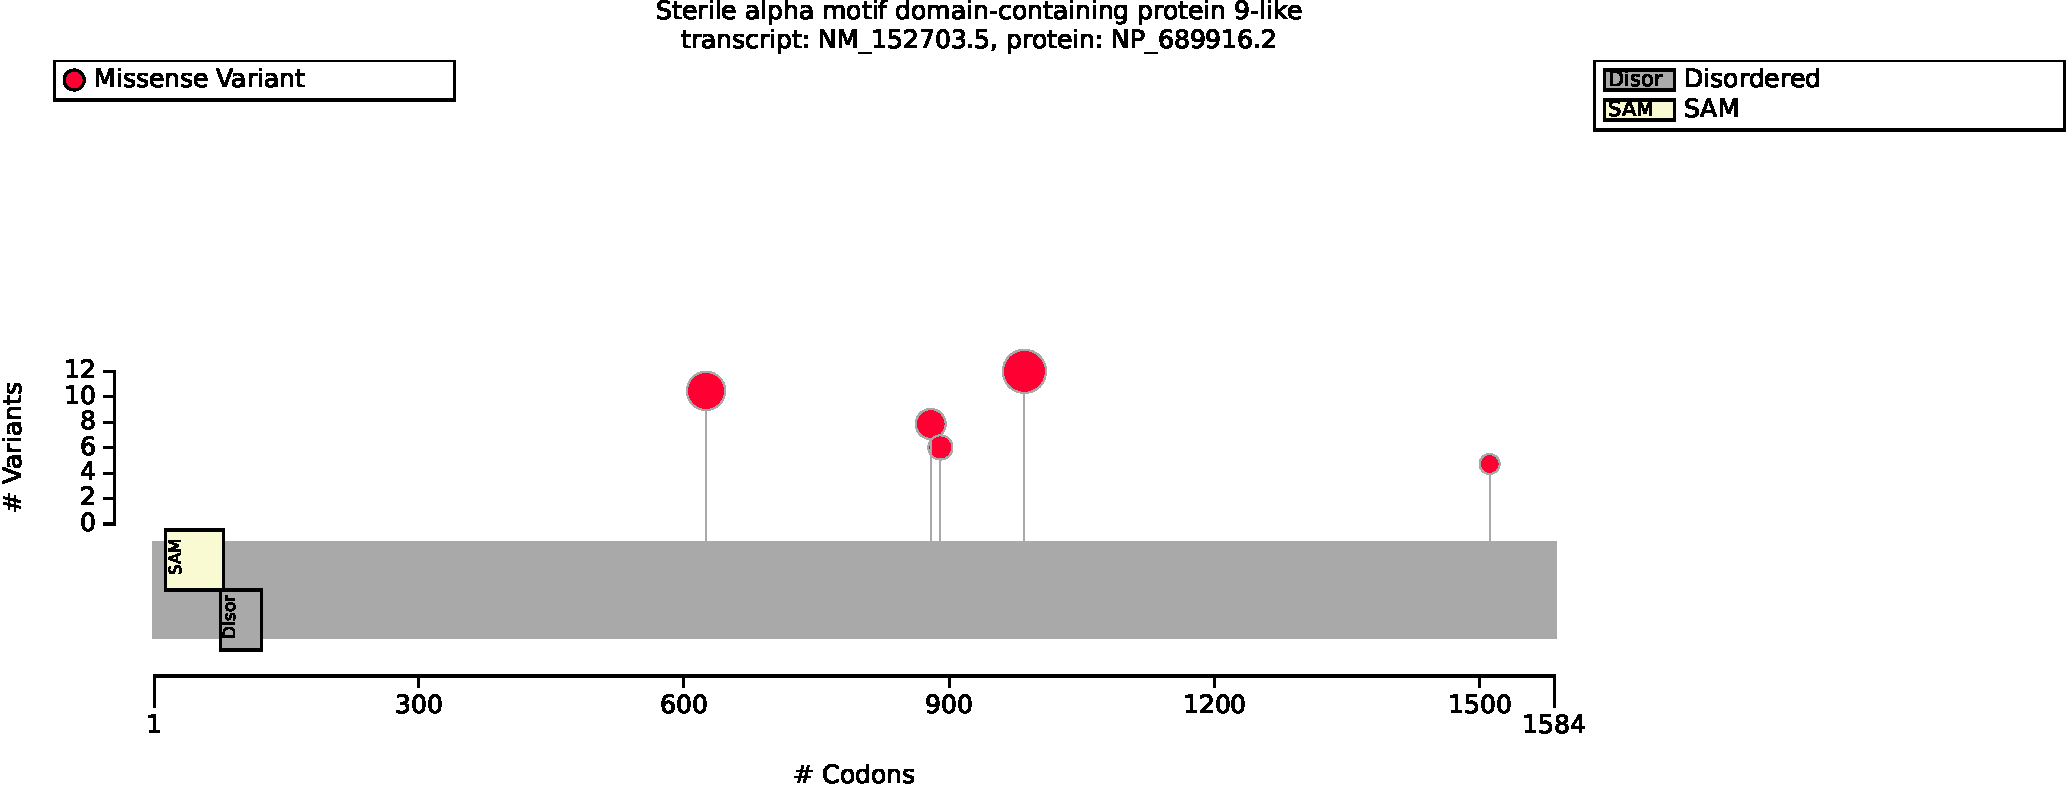
\includegraphics[width=\textwidth]{ img/SAMD9L_protein_diagram.pdf} 
\captionsetup{justification=raggedright,singlelinecheck=false}
\caption{Distribution of variants in SAMD9L}
\end{subfigure}

\vspace{2em}

\begin{subfigure}[b]{0.95\textwidth}
\centering
\resizebox{\textwidth}{!}{
\begin{tabular}{llllrr}
\toprule
HPO term & Arg986Cys & Ser626Leu & p-value & adj. p-value\\
\midrule
Pancytopenia [HP:0001876] & 4/6 (67\%) & 0/9 (0\%) & 0.011 & 0.026\\
Thrombocytopenia [HP:0001873] & 7/9 (78\%) & 0/9 (0\%) & 0.002 & 0.008\\
Neutropenia [HP:0001875] & 7/9 (78\%) & 0/9 (0\%) & 0.002 & 0.008\\
\bottomrule
\end{tabular}
}
\captionsetup{justification=raggedright,singlelinecheck=false}
\caption{         Fisher Exact Test performed to compare HPO annotation frequency with respect to Arg986Cys and Ser626Leu. Total of
        7 tests were performed. }
\end{subfigure}
\vspace{2em}
\begin{subfigure}[b]{0.95\textwidth}
\centering
\resizebox{\textwidth}{!}{
\begin{tabular}{llllrr}
\toprule
Genotype (A) & Genotype (B) & total tests performed & significant results\\
\midrule
N Term & other & 16 & 0\\
\bottomrule
\end{tabular}
}
\captionsetup{justification=raggedright,singlelinecheck=false}
\caption{             Fisher Exact Test performed to compare HPO annotation frequency with respect to genotypes. }
\end{subfigure}

\vspace{2em}

\caption{ The cohort comprised 31 individuals (15 females, 16 males). 5 of these individuals were reported to be deceased. A total of 41 HPO terms were used to annotate the cohort. Disease diagnoses: Ataxia-pancytopenia syndrome (OMIM:159550) (22 individuals), Spinocerebellar ataxia 49 (OMIM:619806) (9 individuals). A recent summary of SAMD9L variants stated there was no evidence of phenotype–genotype correlation \cite{PMID_38594844}.
 A total of 6 unique variant alleles were found in \textit{SAMD9L} (transcript: \texttt{NM\_152703.5}, protein id: \texttt{NP\_689916.2}).}
\end{figure}
